\chapter{Convolutional neural networks (CNN)}\label{ch-16}

Neural networks have a huge number of successful applications, thanks
to their performance and to the fact that they are easily set up as a
first approach for learning arbitrary functions of unknown form,
without assuming an a priori statistical model. \textbf{Sub-symbolic}
tasks (sensory data, motor control, visual processing) are their
workhorse.

This lecture presents a historical and paradigmatic example:
\textbf{convolutional networks} (CNN, \emph{ConvNet}, \emph{LeNet}). It
shows the \textbf{flexibility in the design} of networks, how the
design is changed to deal with a specific application, and how a
\textbf{not fully connected} feedforward network is built for a precise
problem. CNNs are also a historical instance of a \textbf{deep}
network, and they act as a bridge towards deep learning.

\section{The problem: recognising
characters}\label{il-problema-riconoscere-caratteri}

\begin{figure}[htbp]
\centering
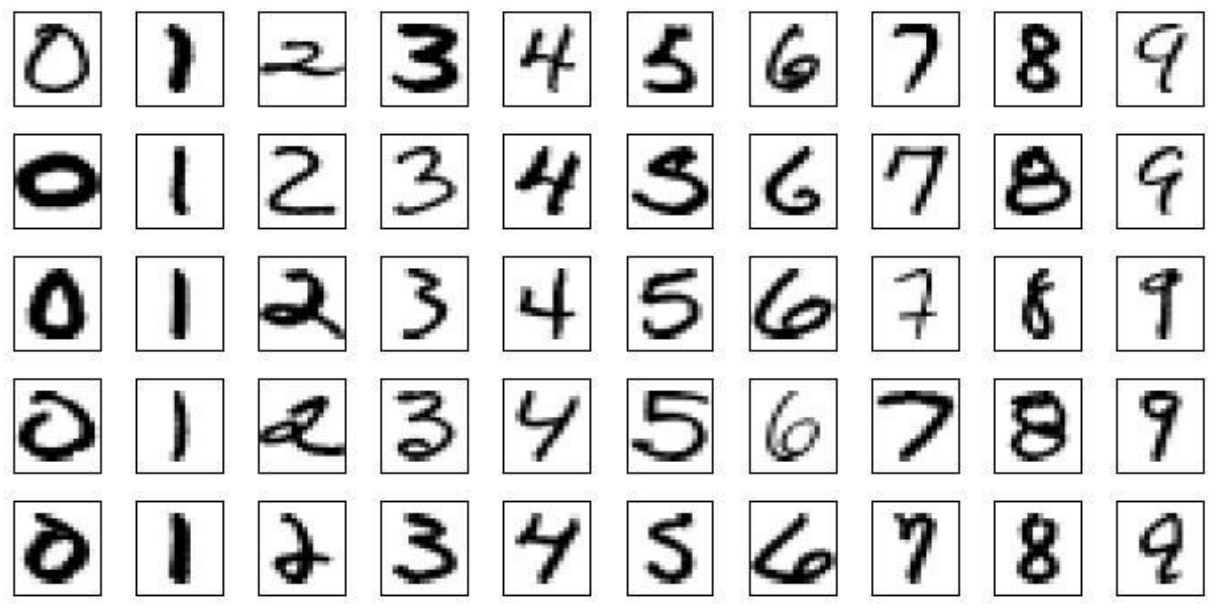
\includegraphics[width=0.69\linewidth,height=0.42\textheight,keepaspectratio]{images/16-cnn_zip.png}
\caption{Examples from the ZIP code dataset: normalised 16×16 8-bit
grey-scale images (Le Cun et al., 1990). The MNIST benchmark is ``the
drosophila of ML''.}
\end{figure}

A first approach is a standard network with \textbf{256 inputs} (one
per pixel, \(16 \times 16\)): an error of 5--20\% is obtained, with
many errors due to the \textbf{lack of invariance} to rotations,
translations, etc. A fully connected network treats each pixel as an
independent input: it does not ``know'' that nearby pixels are
correlated nor that the same stroke can appear in different positions.

\begin{boxtip}{The basic idea}

Exploit the \textbf{architecture} to include \textbf{prior knowledge}
in the network: - \textbf{local connections} (local receptive fields):
each unit sees only a small area of the image, and extracts
\textbf{local features}; - \textbf{weight sharing} among different
units: the \textbf{same operation} is applied to different parts of the
input, because the features of a character can appear anywhere in the
image (regardless of position, small rotations\ldots). The number of
free parameters is reduced while keeping a complex connectivity.

\end{boxtip}

\section{Convolution}\label{la-convoluzione}

The name comes from the \textbf{convolution operator}: a weighted
average of a function \(f\), weighted by another function \(g\) that
slides over time: \[
(f * g)(t) = \int_{-\infty}^{\infty} f(\tau)\,g(t - \tau)\,d\tau.
\] The support of \(g\) is bounded (non-zero only on an interval):
\(g\) acts as a \textbf{sliding window}.

\subsection{1D convolution: a unit on a
stream}\label{convoluzione-1d-una-unituxe0-su-uno-stream}

A unit with three weights sliding over an input sequence: \[
out_t = \sum_{i=1}^{3} w_i\,x_{t+i-2}.
\]

\begin{figure}[htbp]
\centering
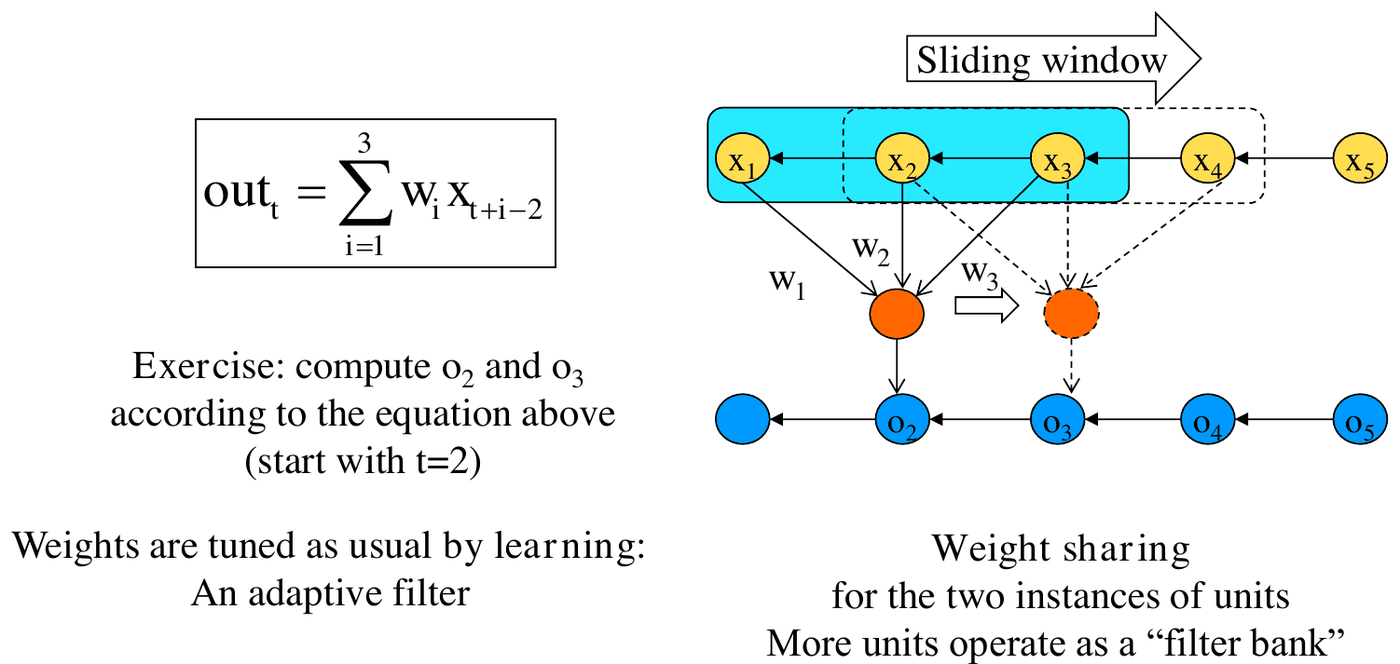
\includegraphics[width=0.80\linewidth,height=0.42\textheight,keepaspectratio]{images/16-cnn_conv1d.png}
\caption{1D convolution: the same unit (with the same weights) slides
over the input.}
\end{figure}

(Exercise: with \(t = 2\), \(o_2 = w_1x_1 + w_2x_2 + w_3x_3\); with
\(t = 3\), \(o_3 = w_1x_2 + w_2x_3 + w_3x_4\).) The weights are
\textbf{shared} among the instances of the unit and are learned as
usual: the unit is an \textbf{adaptive filter}. Several different units
form a \textbf{filter bank}. This network is also called a
\emph{Time-Delay Neural Network}.

\subsection{2D convolution}\label{convoluzione-2d}

On an image a 2D \textbf{kernel} is used, for example \(3 \times 3\)
(the \textbf{local receptive field} of the unit), which moves one pixel
at a time (\textbf{stride} 1). \textbf{Padding} handles the borders.
The kernel slides over the image and produces a \textbf{feature map}
(the features extracted by the filter).

In neural network terms: the image is scanned with \textbf{the same
neuron}, which uses local connections.

\begin{figure}[htbp]
\centering
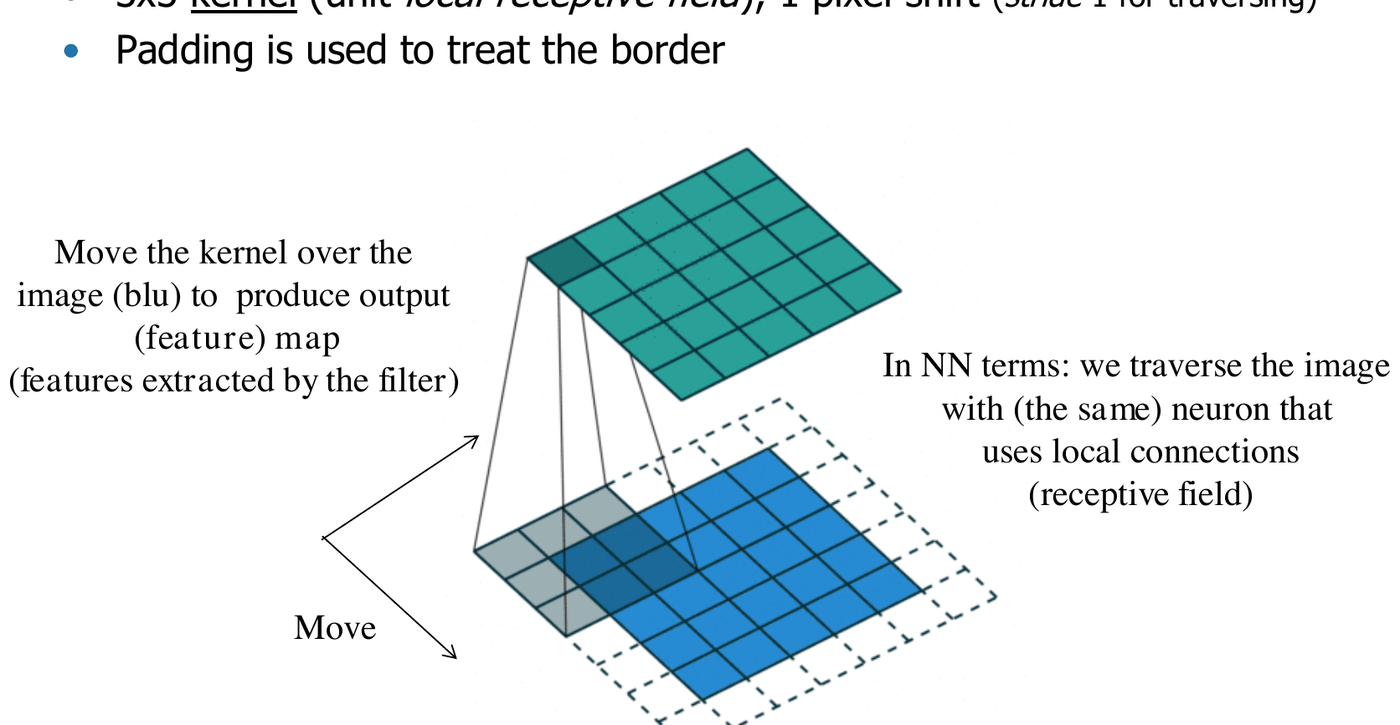
\includegraphics[width=0.80\linewidth,height=0.42\textheight,keepaspectratio]{images/16-cnn_conv2d.png}
\caption{2D convolution: the kernel slides over the image and produces
the feature map.}
\end{figure}

\begin{figure}[htbp]
\centering
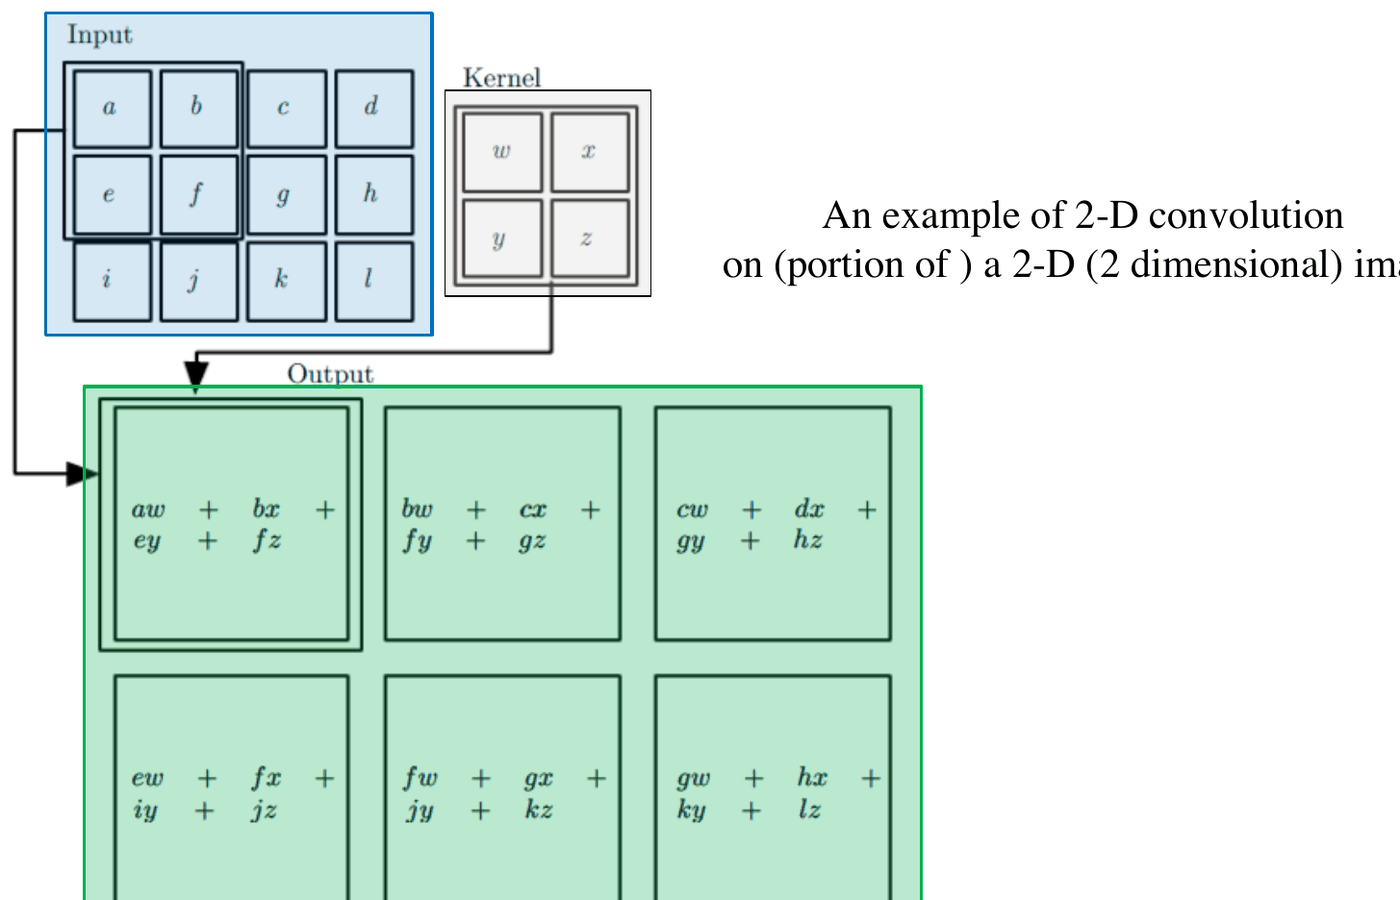
\includegraphics[width=0.66\linewidth,height=0.42\textheight,keepaspectratio]{images/16-cnn_conv2d-esempio.png}
\caption{Example of 2D convolution of a 3×4 input with a 2×2 kernel.}
\end{figure}

\begin{boxnote}{Form used in libraries}

The 2D convolution of an image \(I\) with a kernel \(K\) is
\(S(i,j) = (I * K)(i,j) = \sum_m\sum_n I(m,n)\,K(i-m, j-n)\). Many CNN
libraries actually implement \textbf{cross-correlation}:
\(S(i,j) = \sum_m\sum_n I(i+m, j+n)\,K(m,n)\) (for details: \emph{Deep
Learning book}, sec.\ 9.1; not required for the oral exam).

\end{boxnote}

\subsection{Stride greater than 1}\label{stride-maggiore-di-1}

With \textbf{stride} \textgreater{} 1 the kernel ``skips'' pixels (for
example two at a time): it is a \textbf{sub-sampling}, and it produces
a reduced feature map.

\begin{figure}[htbp]
\centering
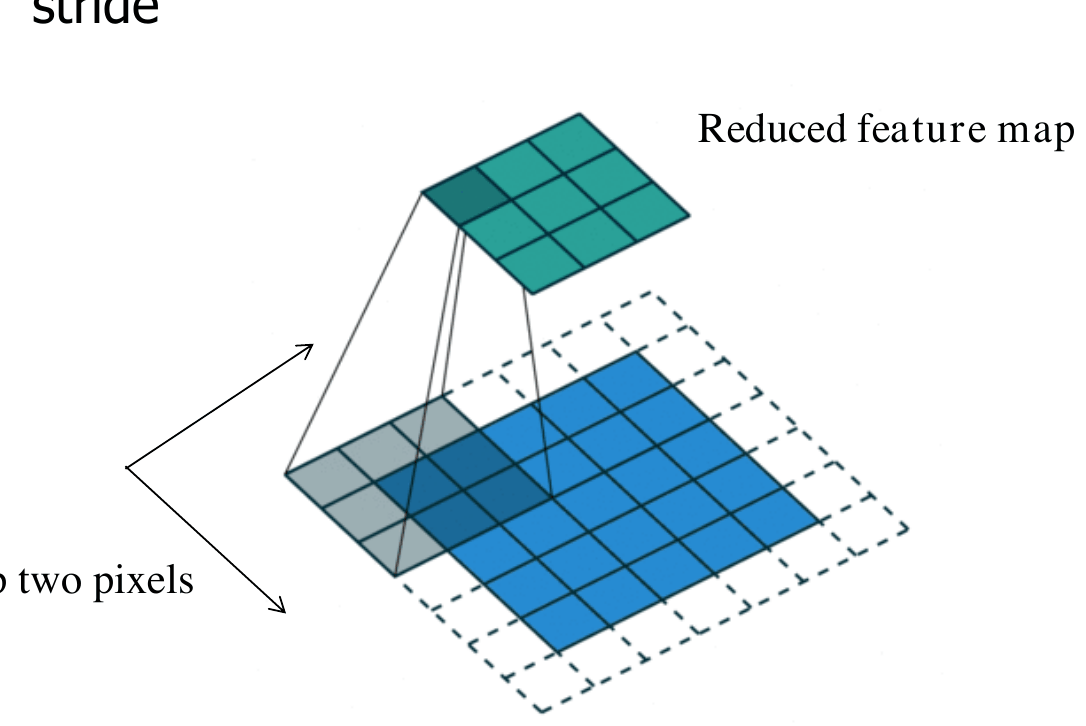
\includegraphics[width=0.51\linewidth,height=0.42\textheight,keepaspectratio]{images/16-cnn_stride.png}
\caption{Convolution with stride 2: the resulting feature map is
reduced.}
\end{figure}

\section{A network of ``filters''}\label{una-rete-di-filtri}

The weights of the units are a \textbf{trained filter} that detects
certain features or patterns in the image. The architecture design
provides:

\begin{itemize}
\tightlist
\item
  \textbf{small, local receptive field}: thanks to this constraint, the
  learned filters respond maximally to \textbf{spatially local}
  patterns (as in the visual cortex of animals);
\item
  \textbf{the same filter applied over the whole image}: features are
  detected \textbf{regardless of position}, obtaining
  \textbf{translation invariance};
\item
  \textbf{learned filters}: the filters that in traditional image
  processing algorithms were designed by hand are \textbf{learned}.
  Independence from prior knowledge and from human effort in designing
  features is a great advantage;
\item
  \textbf{many stacked layers}: the units of the feature maps represent
  increasingly larger areas of the original image (by assembling areas
  of the previous maps).
\end{itemize}

\section{Pooling}\label{pooling}

\textbf{Pooling} reduces the feature map:

\begin{itemize}
\tightlist
\item
  with sub-sampling (stride \textgreater{} 1, seen above);
\item
  with an \textbf{average} (simple or weighted);
\item
  with \textbf{max pooling} (the most common).
\end{itemize}

In practice, instead of producing a value for each input pixel, one is
produced for a (rectangular) set of pixels, taking the mean or the
maximum of the outputs.

\begin{figure}[htbp]
\centering
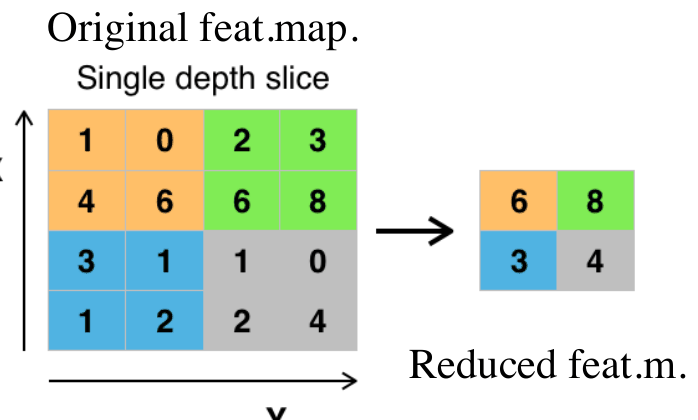
\includegraphics[width=0.40\linewidth,height=0.42\textheight,keepaspectratio]{images/16-cnn_maxpool.png}
\caption{Max pooling with a 2×2 filter and stride 2.}
\end{figure}

Pooling also helps make the representation \textbf{approximately
invariant to small translations} of the input: the maximum (or the
mean) changes little if the input shifts slightly, so a high output
stays high for a slightly translated version.

\section{The CNN as a whole}\label{la-cnn-nel-complesso}

A CNN exploits weight sharing to implement a sliding window of local
fields over a signal, extended to 2D images and repeated over many
layers (feature maps), alternated with pooling operations. The four
ingredients:

\begin{enumerate}
\def\labelenumi{\arabic{enumi}.}
\tightlist
\item
  \textbf{local connections};
\item
  \textbf{shared weights};
\item
  \textbf{pooling};
\item
  \textbf{many layers}.
\end{enumerate}

\begin{figure}[htbp]
\centering
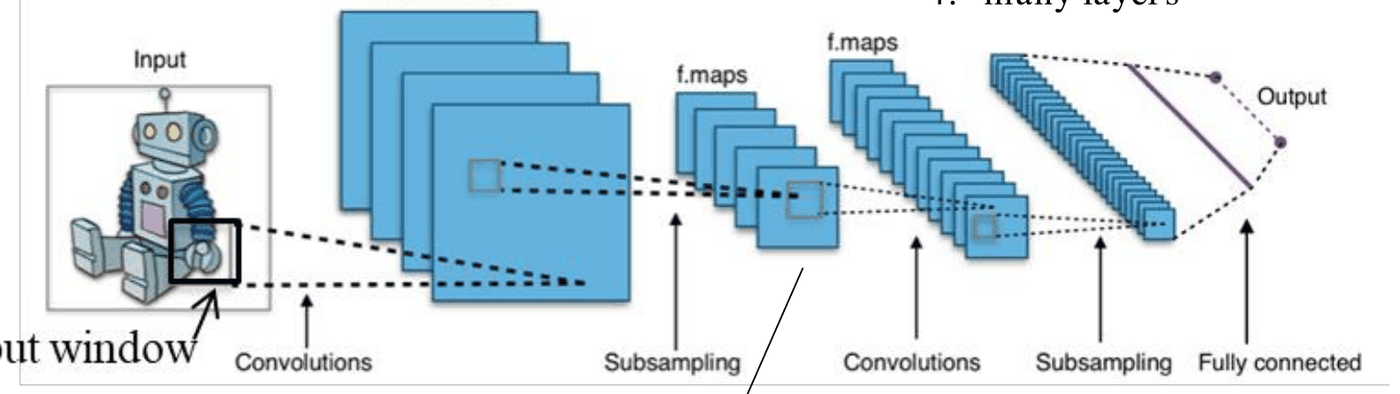
\includegraphics[width=0.89\linewidth,height=0.42\textheight,keepaspectratio]{images/16-cnn_cnn-intera.png}
\caption{A complete CNN: alternating convolutions and sub-samplings,
followed by fully connected layers. The number of filters (feature maps)
can grow in the higher layers.}
\end{figure}

\begin{figure}[htbp]
\centering
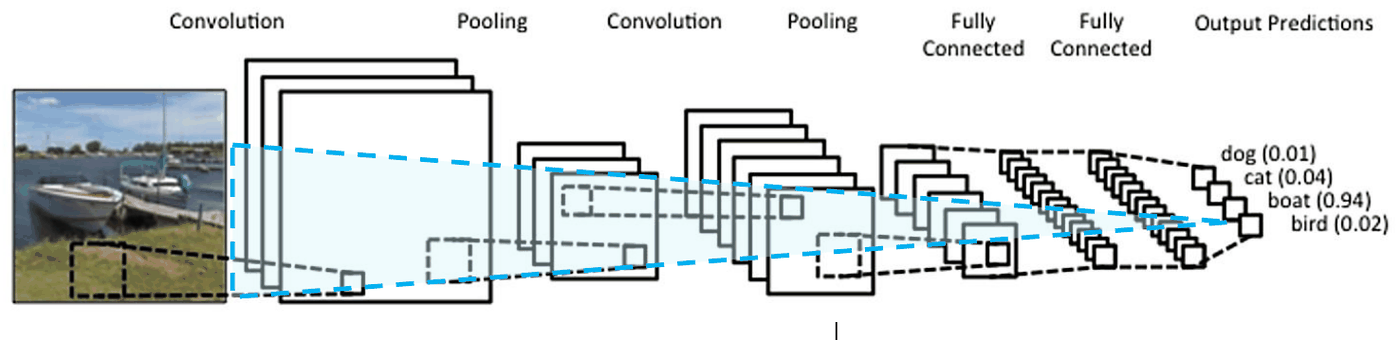
\includegraphics[width=0.89\linewidth,height=0.42\textheight,keepaspectratio]{images/16-cnn_esempio2.png}
\caption{The ``cone'' from the image to the final maps: the receptive
field of the final units is much wider than that of the units of the
first layers, because they are indirectly connected to a large part of
the image.}
\end{figure}

\begin{figure}[htbp]
\centering
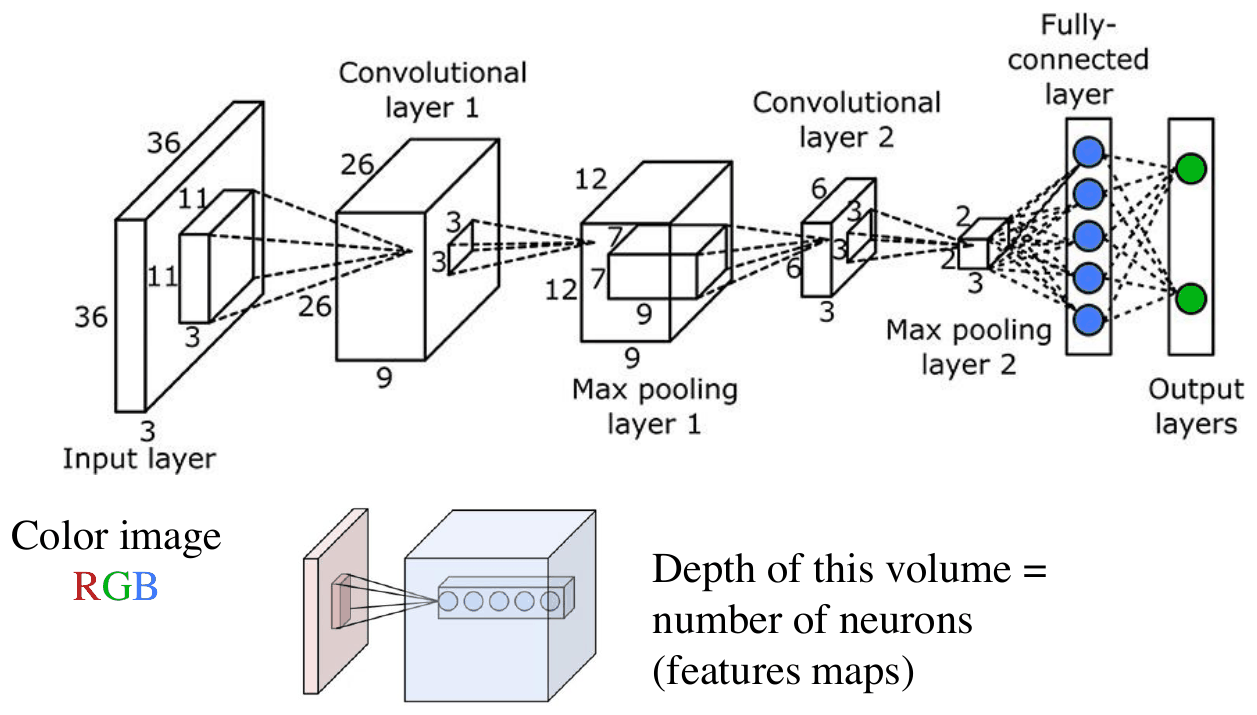
\includegraphics[width=0.71\linewidth,height=0.42\textheight,keepaspectratio]{images/16-cnn_esempio3.png}
\caption{An example with the dimensions; for a colour (RGB) image the
depth of the volume is the number of feature maps.}
\end{figure}

\begin{figure}[htbp]
\centering
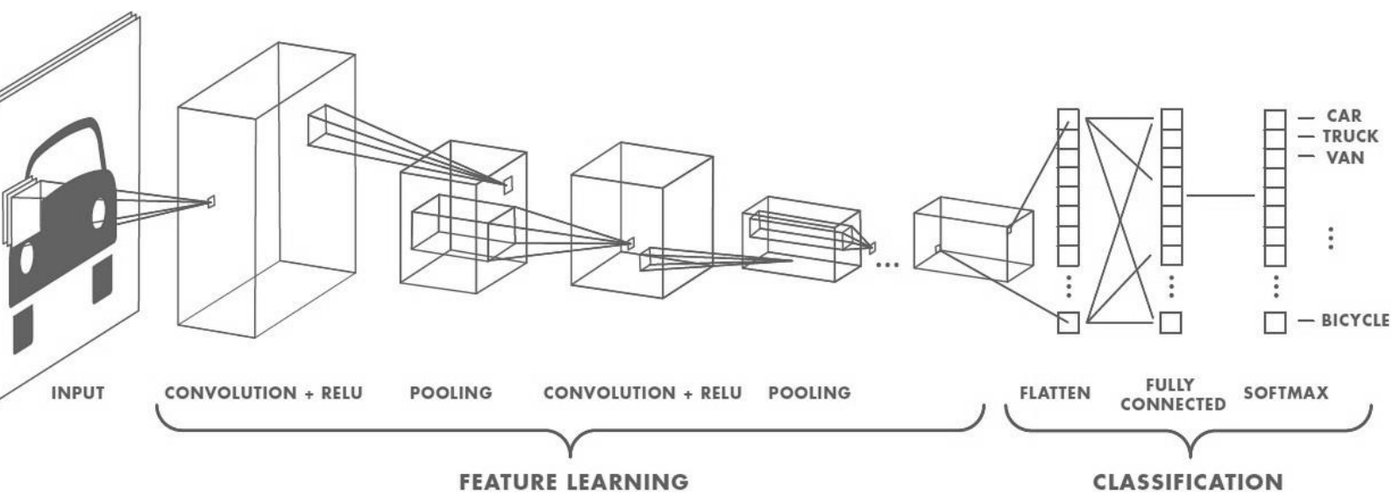
\includegraphics[width=0.89\linewidth,height=0.42\textheight,keepaspectratio]{images/16-cnn_alexnet.png}
\caption{An AlexNet-like architecture.}
\end{figure}

\begin{boxabstract}{Advantages of CNNs}

\begin{itemize}
\tightlist
\item
  \textbf{Local connections and shared weights}: they detect local
  motifs/patterns in images, in a \textbf{translation-invariant} way
  (with respect to the position of the pattern); they \textbf{reduce
  the number of free parameters} while keeping the connections, which
  is a form of \textbf{regularisation}.
\item
  \textbf{Pooling}: reduces the size of the representation at each
  layer (a \textbf{pyramid} of layers) and helps invariance to small
  shifts and distortions.
\item
  \textbf{Many layers}: operations 1 and 2 applied to all the feature
  maps produce a \textbf{progressive abstraction} of the features,
  making it possible to \textbf{compose primitives} (low-level
  features, learned only once) in all possible combinations in the
  subsequent layers.
\item
  They are a historical instance of a \textbf{deep network}, and
  analogies with the visual system have been studied (neuroscience).
\end{itemize}

\end{boxabstract}

\section{How they are used}\label{come-si-usano}

Training is typically done with \textbf{backpropagation}, with the
well-known heuristics and some specialisations (for weight sharing,
pooling\ldots). Given the typical use of huge networks and large
amounts of data, many hyperparameters are fixed \textbf{by experience}
or on the advice of experts, because it would be too expensive to
cross-validate over large hyperparameter spaces. Training,
regularisation effects and the good behaviour of these huge networks
will be discussed in the framework of deep learning.

\section{Historical results}\label{risultati-storici}

\subsection{LeCun's architectures on the ZIP code
dataset}\label{le-architetture-di-lecun-sul-dataset-zip-code}

\begin{figure}[htbp]
\centering
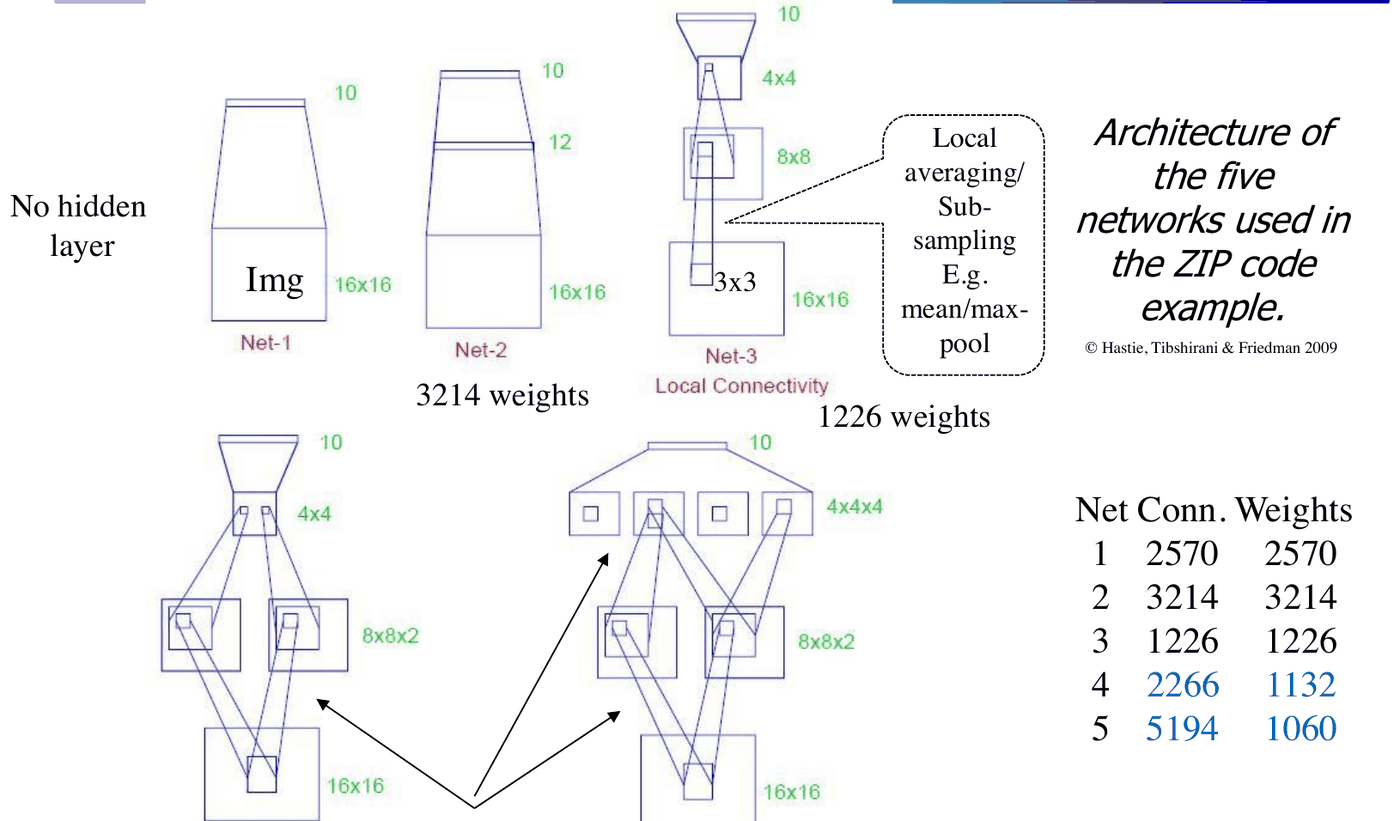
\includegraphics[width=0.89\linewidth,height=0.42\textheight,keepaspectratio]{images/16-cnn_lecun.png}
\caption{The five networks used by LeCun on the ZIP code problem: from a
network without hidden layers (Net-1) to networks with local
connections (Net-3) and shared weights (Net-4, Net-5).}
\end{figure}

{\def\LTcaptype{none} % do not increment counter
\begin{longtable}[]{@{}lll@{}}
\toprule\noalign{}
Network & Connections & Weights \\
\midrule\noalign{}
\endhead
\bottomrule\noalign{}
\endlastfoot
Net-1 & 2570 & 2570 \\
Net-2 & 3214 & 3214 \\
Net-3 & 1226 & 1226 \\
Net-4 & 2266 & 1132 \\
Net-5 & 5194 & 1060 \\
\end{longtable}
}

With shared weights the number of \textbf{connections} can grow while
the number of \textbf{weights} (free parameters) stays low.

\begin{figure}[htbp]
\centering
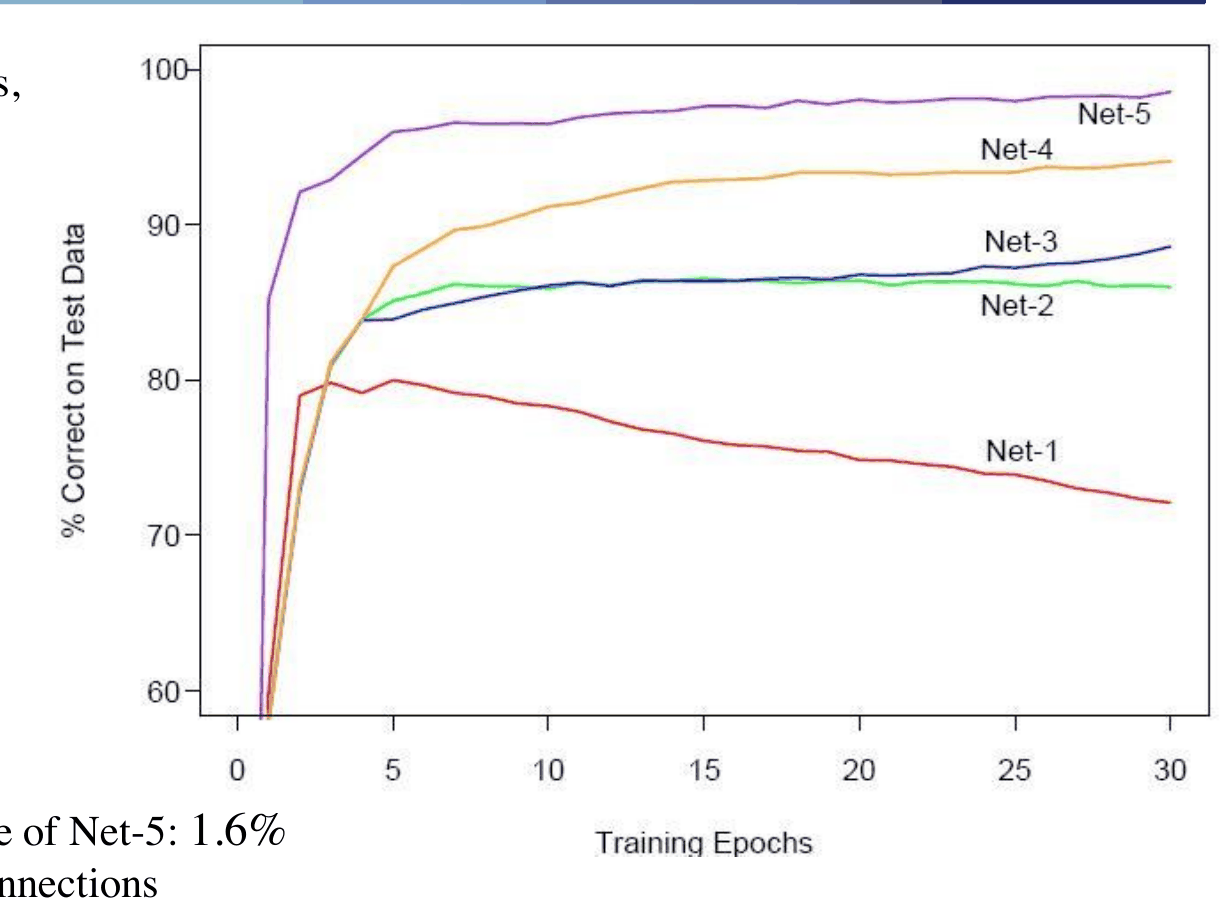
\includegraphics[width=0.63\linewidth,height=0.42\textheight,keepaspectratio]{images/16-cnn_lecun-curve.png}
\caption{Test performance curves for the five networks (Le Cun, 1989).
The training error is zero for all of them, on a reduced set of about
300 images.}
\end{figure}

Net-5 reaches an error of \textbf{1.6\%} with 5194 connections and only
1060 weights. Today 0.8\% (with networks and SVMs) and even less is
achieved.

\subsection{MNIST}\label{mnist}

The complete dataset has 60,000 training images and 10,000 test images.
Progress (1998--2012) is documented on LeCun's website. With deep
learning (MLPs or CNNs with many layers, unsupervised layer-wise
pre-training) 0.39\% (2006) and 0.35\% (2011) were reached; the best in
2012 is 0.23\% (committee of convolutional networks), 0.21\% in 2016.

\begin{boxwarning}{Warning}

The MNIST test set has been used so many times that improvements of
the order of 0.1\% are no longer significant: it has de facto become a
validation set for the community.

\end{boxwarning}

\begin{boxnote}{Does a deep MLP work too?}

A 2010 paper (\emph{Neural Computation}) shows that ``good old''
on-line backpropagation on a simple MLP achieves 0.35\% on MNIST: all
that is needed is \textbf{many layers}, \textbf{many neurons} per
layer, \textbf{many deformed images} for training and \textbf{GPUs} to
speed things up. The 784-2500-2000-1500-1000-500-10 network has 12
million weights and trains in 2 hours. Complexity control is obtained
by deforming the images to have many more examples (\emph{data
augmentation}).

\end{boxnote}

\subsection{Face recognition and
ImageNet}\label{riconoscimento-facciale-e-imagenet}

\begin{itemize}
\tightlist
\item
  \textbf{DeepFace} (CVPR 2014): 9-layer convolutional networks trained
  on 4 million images of more than 4000 people; it recognises whether
  two photos show the same person with 97.25\% accuracy (humans:
  97.53\%).
\item
  \textbf{AlexNet} (Krizhevsky, Sutskever, Hinton, NIPS 2012): a deep
  CNN trained on 1.3 million high-resolution images from ImageNet
  (ILSVRC-2010) in 1000 classes. Top-1 and top-5 errors of 39.7\% and
  18.9\% (from the previous \textasciitilde26\%), much better than the
  state of the art. The network has \textbf{60 million parameters} and
  500,000 neurons: five convolutional layers (some followed by max
  pooling) and two fully connected layers with a final 1000-class
  softmax. To speed up training: \textbf{non-saturating} neurons (ReLU)
  and a very efficient GPU implementation. To reduce overfitting in the
  dense layers: a new regularisation method, \textbf{dropout}.
\end{itemize}

\begin{figure}[htbp]
\centering
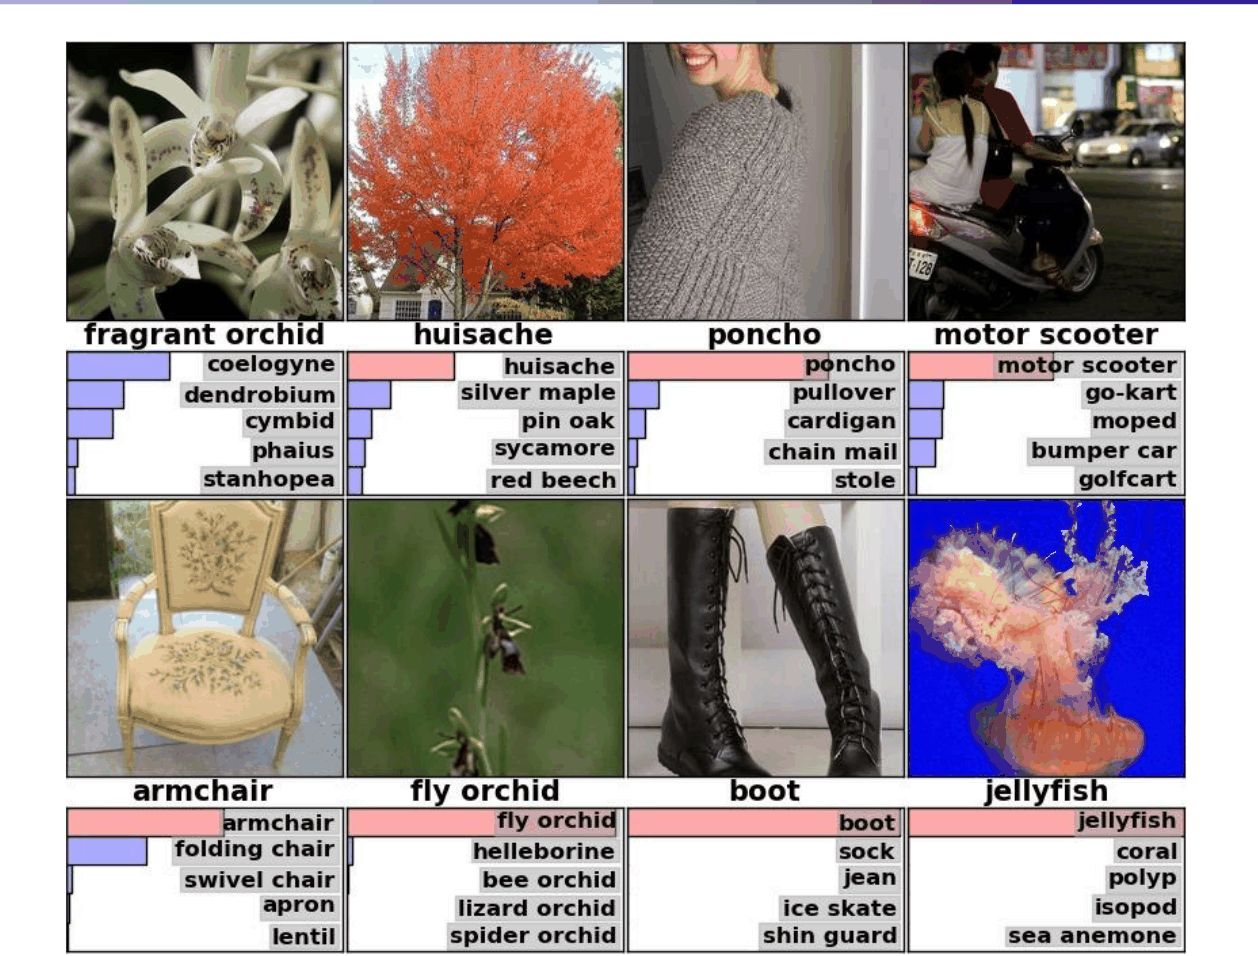
\includegraphics[width=0.63\linewidth,height=0.42\textheight,keepaspectratio]{images/16-cnn_imagenet.png}
\caption{AlexNet top-5 predictions on random test set images.}
\end{figure}

\section{Modern CNNs and GPUs}\label{cnn-moderne-e-gpu}

There are many variants and specialised architectures for images
(course \emph{Intelligent Systems for Pattern Recognition}), with a
great impact on Pattern Recognition and Computer Vision; the
neuroscientific foundations are covered in the \emph{Computational
Neuroscience} course. Features of models \textbf{already trained} on
large benchmarks (AlexNet, GoogLeNet, VGG, ResNet\ldots) can also be
reused: many pre-trained CNNs are available for classification,
segmentation, face recognition, text detection.

Efficient implementations exploit \textbf{GPUs} through the
\textbf{tensor} representation. Matrix multiplication (i.e.\ dot
products) is a linear operation that GPUs perform very efficiently,
parallelising the independent sums and products. Many kernel operations
can be written as a single multiplication between block matrices; the
\textbf{tensor} notation (multidimensional arrays with the
\emph{tensordot} operation, for example in TensorFlow or NumPy) makes
it possible to do so without building complex block matrices by hand.

\begin{boxnote}{Beyond CNNs: Capsule Networks}

\textbf{Capsule Networks} (Sabour, Frosst, Hinton, 2017) use
specialised sub-networks: a ``capsule'' is a group of neurons that
outputs both a parameter indicating whether an entity is present and a
vector of \textbf{pose parameters} (position, orientation) relative to
a canonical version. Instead of max pooling they use a \textbf{routing}
mechanism (the idea that the brain routes low-level visual information
to the most suitable capsule). They achieve excellent results on MNIST,
recognising overlapping digits much better than a CNN.

\end{boxnote}

\begin{boxquestion}{Possible exam questions}

\begin{itemize}
\tightlist
\item
  What are the key ideas of CNNs (local connections, shared weights,
  pooling, many layers) and what does each imply?
\item
  What is convolution in a neural network? What are kernel, stride,
  padding, feature map?
\item
  What is pooling for? How does max pooling work?
\item
  Why is weight sharing a form of regularisation?
\item
  How does the receptive field grow with depth?
\end{itemize}

\end{boxquestion}
